\documentclass[10pt]{beamer}

%%%
% PREAMBLE FOR THIS DOC 
%%%
%https://tex.stackexchange.com/questions/68821/is-it-possible-to-create-a-latex-preamble-header
\usepackage{/Users/miw267/Repos/latex_preamble/beamer_preamble}

\usetikzlibrary{matrix}


%%%
% DOCUMENT
%%%

\begin{document}

%\maketitle

%% Title page frame
%\begin{frame}
%    \titlepage 
%\end{frame}



\title{11/06/2026: Conditional Probability \\ \qquad \qquad \qquad \& Independence }
\author{CSCI 246: Discrete Structures}
\date{Textbook reference: Sec 32, Scheinerman}

\begin{frame}
    \titlepage 
\end{frame}


\begin{frame}


\begin{myyellowbox}[title=Today's Agenda]
\begin{itemize}
	\item Weekly quiz (20-25 mins)
	\item Odds and Ends ($\approx$ 5 mins)
	\item Mini-lecture ($\approx$ 20 mins)
\end{itemize}

\end{myyellowbox}

\end{frame}


\begin{frame}[fragile]
\footnotesize 
 \begin{myredbox}[title=\text{Weekly Quiz \#9}] 
\begin{enumerate}
\item \textit{(Algorithmic Efficiency.)}  For the algorithm segment: (a) Compute the actual number of elementary operations (additions, subtractions, multiplications, divisions, and comparisons) that are performed when the algorithm segment is executed. For simplicity, however, count only comparisons that occur within the body of the for loop. (b) Find the order of the algorithm segment.
	\begin{python}[basicstyle=\ttfamily\scriptsize, numbers=none, columns=fullflexible, keepspaces=true]
for i in range(3, n):
    a = 3*n + 2*i - 1
	\end{python}
\item \textit{(Big O and Big Theta.)}  Let $a_n = n^2 + n + 1 + \frac{1}{n} + \sin n$. Prove that $a_n = O(n^2)$.
\item \textit{(Functions.)}  Let $A$ be the set of even integers and $B$ be the set of odd integers.  Show that the function $f: A \to B$ defined by $f(x)+1$ is a bijection.
\end{enumerate}
\end{myredbox}
\vfill 
\colorbox{green!30}{\textbf{Definition.}} Let $f$ and $g$ be functions. Then $f$ is of order at most $g$, written $f(n)$ is $O(g(n))$ ($f$ of $n$ is big-O of $g$ of $n$) if and only if there exist positive real number $B$ and integer $n_0$ such that
\[  |f(n)| \leq B |g(n)| \quad \text{for every integer } n \geq n_0\]	

%\vfill 
%\begin{mygreenbox}[title=\text{Reference Material: Beginning of Proof by Well-Ordering Principle} }]
%Suppose, for the sake of contradiction, that the statement is false.  Let $X \subseteq \mathbb{N}$ be the set of counterexamples to the statement. Since we have suppp
%\end{mygreenbox}

\end{frame}


\begin{frame}[standout]
Odds and ends from last time
\end{frame}



\begin{frame}
\footnotesize 



 \colorbox{red!30}{\textbf{Question.}}  What is the probability of getting \textbf{two pairs} in a 5-card poker hand?
 \vfill 
  \colorbox{yellow!30}{\textbf{Poll.}} What is the error in the proposed solution below?
 \vfill 
 \pause 
 \colorbox{blue!30}{\textbf{Proposed Solution.}} Let $S$ be the sample space of poker hands. 
 % That is, 
%\[S=\bigg\{ \set{A\spadesuit 2 \spadesuit 3 \spadesuit 4 \spadesuit 5 \spadesuit}, \;   \hdots, \; \set{9 \heartsuit 10 \heartsuit J \heartsuit Q \heartsuit K \heartsuit} \bigg\}. \]
Let $E \subset S$ be the event that the poker hand is two pairs. Then by the equally likely probability formula, 
\begin{align*}
P(E) = 	\frac{|E|}{|S|} = \frac{\text{\# of two pair poker hands}}{\text{\# of poker hands}}
\end{align*}
Now $|S|=\binom{52}{5} =  2,598,960$, so we just need to find $|E|$.  We proceed in steps:

\begin{enumerate} \footnotesize 
\item \textbf{Choose the rank} for the first pair 	(e.g., two Kings or two 7s).  There are 13 possible ranks.
\item \textbf{Select 2 of the 4 suits} for that rank:  $\binom{4}{2}=6$.
\item \textbf{Choose the rank} for the second pair.  There are 12 ranks which differ from the first pair rank.
\item \textbf{Select 2 of the 4 suits} for that rank:  $\binom{4}{2}=6$.
\item \textbf{Choose the rank} for the fifth card.  There are 11 ranks which differ from those of the two pairs.
\item \textbf{Select 1 of the 4 suits} for that rank:  $\binom{4}{1}=4$.
\item \textbf{Combine the choices}:  $|E|=13 \times 6 \times 12 \times 6 \times 11 \times 4 = 123,552$.
\end{enumerate}
\vspace{-.1cm}
\pause 
 \colorbox{green!30}{\textbf{Corrected Solution.}} The proposed solution has $\binom{13}{1} \binom{12}{1} = (13)(12) = (13)_2$.   The correct answer should be $\binom{13}{2} = \frac{(13)(12)}{2}$.  The proposed solution assumes order matters, which it doesn't in poker hands.  E.g. $\set{K,K,Q,Q,A} = \set{Q,Q,K,K,A}$.   
\end{frame}


\begin{frame}[standout]
Mini-lecture: conditional probability 
\end{frame}


\begin{frame}

\begin{myyellowbox}[title=\text{Practice Reading Quiz (Conditional Probability and Independence)}]


Let $A$ and $B$ be events in a probability space $(S,P)$.  

\vspace{.2cm}

Suppose $P(B) = \frac{1}{2}$ and $P(A \cap B) = \frac{1}{8}$.  

\vspace{.2cm}

Compute $P(A \cond B)$.
%\item Let $A$ and $B$ be events in a probability space $(S,P)$.  Under what condition does
%\[ P(A \cap B) = P(A) P(B)?\]


\end{myyellowbox}
	
\vfill 
\pause

%\begin{mygreenbox}[title=\text{Definition}]
%Let $A$ and $B$ be events in a probability space $(S,P)$, and suppose $P(B) \neq 0$.  Then the \textbf{conditional probability} $ P(A \cond B)$, the probability of $A$ given $B$, is 
%\[ P(A \cond B) = \frac{P(A \cap B)}{ P(B)} \]
%\end{mygreenbox}
%
%	
%\vfill 
%\pause

\colorbox{green!30}{\textbf{Solution.}} By the definition, the solution to the reading quiz is
\[P(A \mid B) = \frac{1/8}{1/2} =  \frac{1}{4}. \]

\vfill 
\pause

\colorbox{red!30}{\textbf{Help!}} How does this make sense?! 
\end{frame}

\begin{frame}{Conditional probability: The idea}
	
Let $U$ be the \textbf{sample space} (the space of all possible outcomes).
\begin{figure}
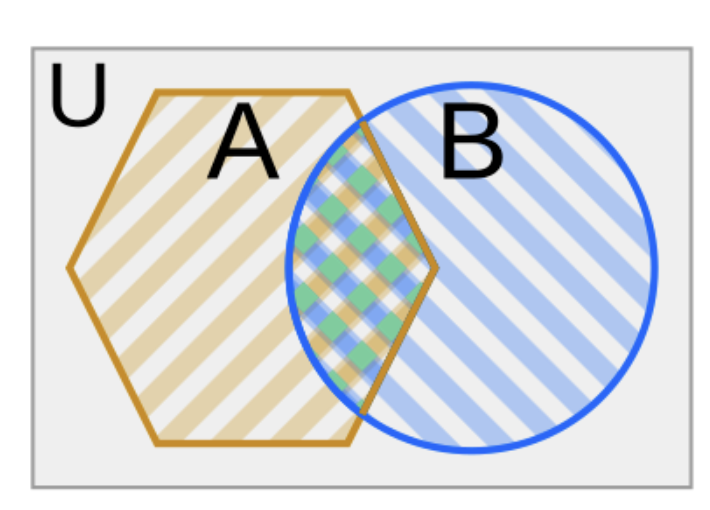
\includegraphics[width=.4\textwidth]{images/the_idea_of_conditional_prob_1.png}	
\end{figure}

\begin{figure}
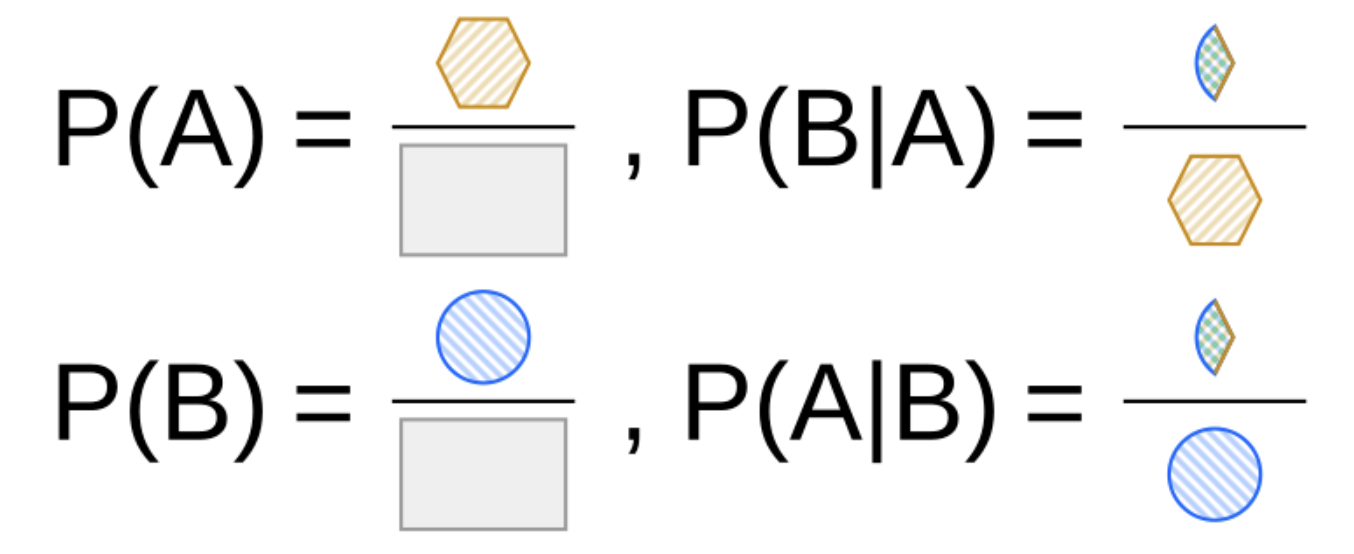
\includegraphics[width=.4\textwidth]{images/the_idea_of_conditional_prob_2.png}	
\end{figure}


\vfill
\pause 
\colorbox{yellow!30}{\textbf{Poll.}} What does  $P(A \mid B)$ mean?
\vfill
\pause 
\colorbox{green!30}{\textbf{Solution.}}
$P(A \mid B)$ means: if you \textbf{know} that $B$ happened, what's the probability that $A$ \textbf{also} happened?	
\end{frame}



\begin{frame}{Conditional probability}
\footnotesize 
\begin{mygreenbox}[title=\text{Definition}]
Let $A$ and $B$ be events in a probability space $(S,P)$, and suppose $P(B) \neq 0$.  Then the \textbf{conditional probability} $ P(A \cond B)$, the probability of $A$ given $B$, is 
\[ P(A \cond B) = \frac{P(A \cap B)}{ P(B)} \]
\end{mygreenbox}
\vfill 
\pause 
\begin{myredbox}[title=Example]

\begin{minipage}{.45\textwidth}
Let $A$ be the event of a student missing the school bus, and $B$ be the event that the student's alarm clock malfunctions. \\

Both events are rare.  But the conditional probability $P(A \cond B)$ is high.  It can be interpreted as follows: if we shrink the underlying sample space from $S$  to the event $B$, what proportion of the little black square $P(B)$ is covered by the shaded area $P(A \cap B)$? 
\end{minipage} %
\hfill 
\begin{minipage}{.45\textwidth}
\begin{figure}
\begin{center}
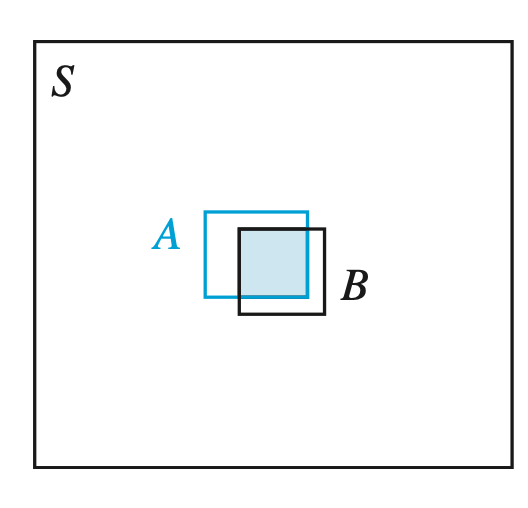
\includegraphics[width=.6\textwidth]{images/conditional_prob.png}
\end{center}
%	
\footnotesize \textbf{Figure 2:} Probability of events $A$, $B$, and $A \cap B$, given as areas. Here we assume that the sample space $S$ has area 1.
\end{figure}
\end{minipage} %
   
\end{myredbox}

\end{frame}


\begin{frame}

\begin{mybluebox}[title=\text{Interpretation of $P(A|B)$}]
If you sample an outcome from the sample space $S$ and you \textbf{know} it's in $B$, then what's the probability that it's \textbf{also} in $A$?
\end{mybluebox}

\end{frame}



\begin{frame}
\Large 

\colorbox{red!30}{\textbf{Remark:}} \; Misunderstandings about conditional probability underly some of the most fundamental and important mistakes in human reasoning!


\end{frame}

\begin{frame}{Base rate fallacy}
\small
\colorbox{green!30}{\textbf{Example: Infectious disease test.}} Let $\mathcal{I}$ be the event that a person is infected with a disease, and $\mathcal{P}$ be the event that the person tests positive for the disease.

Suppose we collect the following data:
%
\begin{center}
\begin{tabular}{|>{\columncolor[gray]{0.85}}c|>{\columncolor[gray]{0.85}}c|>{\columncolor[gray]{0.85}}c|>{\columncolor[gray]{0.85}}c|}
\hline
\rowcolor[gray]{0.85}
\textbf{Number of people} & \textbf{Infected} & \textbf{Uninfected} & \textbf{Total} \\
\hline
\cellcolor[gray]{0.85}\textbf{Test positive}  & \cellcolor[gray]{0.95} 20  & \cellcolor[gray]{0.95} 450 & \cellcolor[gray]{0.95} 470 \\
\hline
\cellcolor[gray]{0.85}\textbf{Test negative}  & \cellcolor[gray]{0.95} 0  & \cellcolor[gray]{0.95}9530  & \cellcolor[gray]{0.95}9530 \\
\hline
\cellcolor[gray]{0.85}\textbf{Total}          & \cellcolor[gray]{0.95} 20                 & \cellcolor[gray]{0.95} 9980                 & \cellcolor[gray]{0.95}10000 \\
\hline
\end{tabular}
\end{center}


The test is very accurate:
%
\begin{align*}
P(\mathcal{P} \cond \mathcal{I}) = \frac{P(\mathcal{I} \cap \mathcal{P})}{P(\mathcal{I})}  = \frac{20}{20} = 1.0, \qquad P(\overline{\mathcal{P}} \cond \overline{\mathcal{I}}) = \frac{P(\overline{\mathcal{I}} \cap \overline{\mathcal{P}})}{P(\overline{\mathcal{I}})}=  \frac{450}{9980} = 0.955
\end{align*}
%
\only<2>{\colorbox{yellow!30}{\textbf{Poll.}} If you test positive, how likely are you to have the disease?}
%
\only<3->{But the probability of having the disease if you test positive is very low!}

\only<4->{%
\begin{align*}
P(\mathcal{I} \cond \mathcal{P}) = \frac{P(\mathcal{I} \cap \mathcal{P})}{P(\mathcal{P})} = \frac{20}{470} \approx .042 
\end{align*}
}
%
\only<5->{
\colorbox{blue!30}{\textbf{Other examples.}} Drunk driving, terrorist identification, \textit{why most published research findings are false.}
}
	
\end{frame}


\begin{frame}{Monte Hall Problem}
\small 
\begin{center}
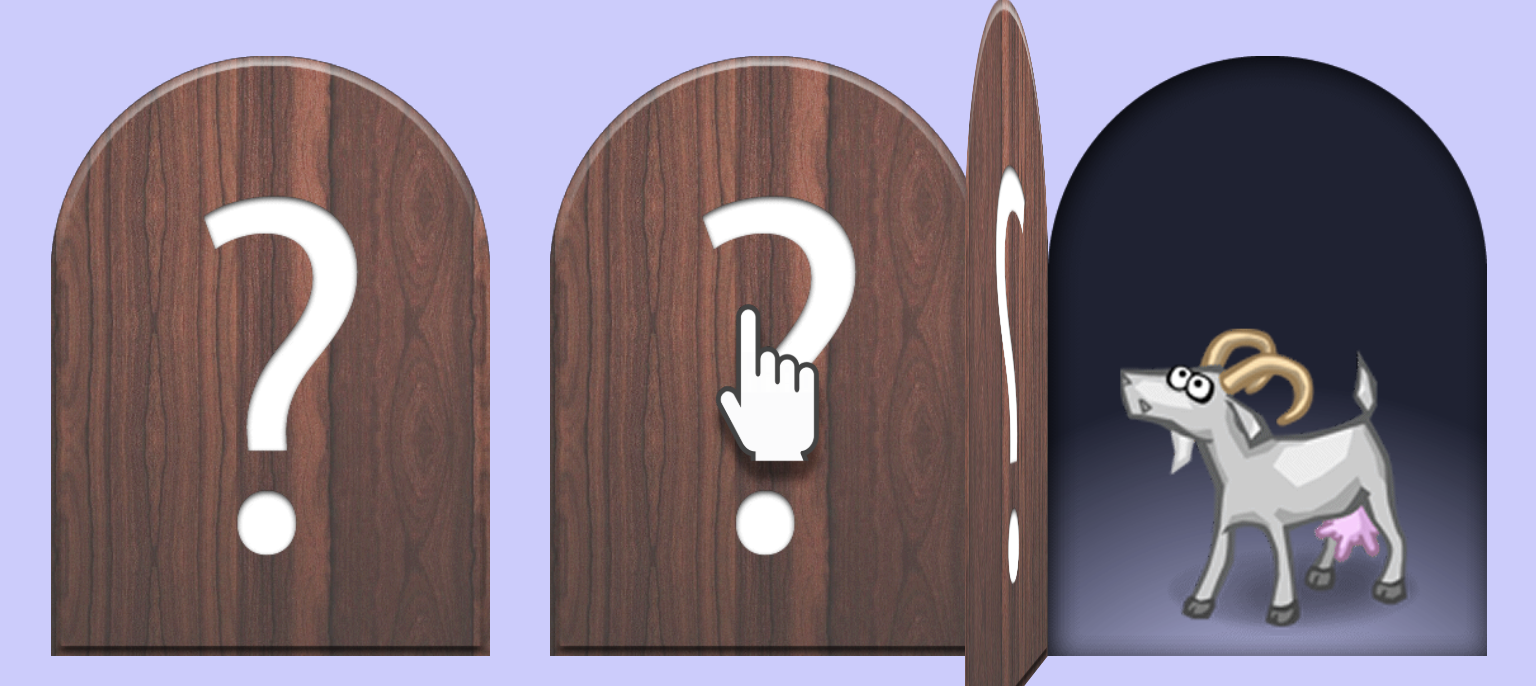
\includegraphics[width=.6\textwidth]{images/monte_hall.png}	
\end{center}

There are three doors on the set for a game show. Behind one door is a car and behind the other two doors are goats. \\
\vfill 

You get to pick a door to open. The host of the show then opens one of the other doors and reveals a goat.  What should you do if you want to maximize your chance of winning the car: stay with your original door  or switch -- or would the likelihood of winning be the same either way?
\vfill \vfill 
%\pause 
%\colorbox{yellow!50}{Try it!} \quad 
%\scriptsize  \url{https://www.mathwarehouse.com/monty-hall-simulation-online/}
\end{frame}

\begin{frame}{Solution to Monte Hall Problem}
\footnotesize 
\colorbox{red!30}{\textbf{A common (and incorrect) analysis.}} Once one door has been revealed, the probability of a car being behind either other door is $\frac{1}{2}$, so it doesn't matter whether you switch or not.
\vfill 
\pause 
\colorbox{green!30}{\textbf{The correct result.}}
We can perform repeated experiments (on a computer or in vivo), and find that the number of wins when switching tends towards $\frac{2}{3}$, and the number of wins when staying tends towards $\frac{1}{3}$.
\pause 
\vfill 
\colorbox{blue!30}{\textbf{Try it!}} \quad 
\scripttext{\url{https://www.mathwarehouse.com/monty-hall-simulation-online/}}
\pause 
\vfill 
\colorbox{yellow!30}{\textbf{Poll.}} What's going on here?
\end{frame}


\begin{frame}
\small
\begin{mybluebox}[title=\text{The Monty Hall Problem}]
A car is behind one of three doors, goats behind the others.  You pick door 1; the host, who knows where the car is, opens door 3 to show a goat.  Should you switch to door 2?
\end{mybluebox}

\onslide<2->{
\colorbox{green!30}{\textbf{Solution.}}
Let $C_i$ = \qq{car is behind door $i$} and $H_3$ = \qq{host opens door 3}.
}

\[
\renewcommand{\arraystretch}{1.1}
\begin{array}{lccc}
\uncover<3->{ & C_1 & C_2 & C_3 \\ \hline}
\uncover<3->{P(C_i)} & \uncover<3->{\frac13} & \uncover<3->{\frac13} & \uncover<3->{\frac13} \\
\uncover<4->{P(H_3 \mid C_i)} & \uncover<5->{\frac12} & \uncover<6->{1} & \uncover<7->{0} \\
\uncover<8->{P(H_3 \cap C_i) = P(H_3 \mid C_i)\,P(C_i)} & \uncover<9->{\frac16} & \uncover<10->{\frac13} & \uncover<11->{0}
\end{array}
\]
%\onslide<4->{{\footnotesize (The host picks door 2 or 3 at random if the car is behind door 1, must pick door 3 if it's behind door 2, and never reveals the car.)}}

\onslide<12->
Since the $C_i$ are disjoint, $P(H_3) = P(H_3 \cap C_1) + P(H_3 \cap C_2) + P(H_3 \cap C_3) = \frac16 + \frac13 + 0 = \frac12$.  

Hence
\[ P(C_2 \mid H_3) = \frac{P(C_2 \cap H_3)}{P(H_3)} = \frac{1/3}{1/2} = \alert{\frac23}
   \quad \text{and} \quad
   P(C_1 \mid H_3) = \frac{1/6}{1/2} = \frac13. \]

\onslide<13->
\textbf{Answer.} Switch!  Switching wins $\frac23$ of the time; staying wins only $\frac13$.
\end{frame}



\begin{frame}{The intuition}
%\footnotesize 
%\colorbox{red!30}{A common (and incorrect) analysis.} Once one door has been revealed, the probability of a car being behind either other door is $\frac{1}{2}$, so it doesn't matter whether you switch or not.
%\vfill 
%\pause 
%\colorbox{green!30}{The correct analysis.}
\vspace{-0.3cm}
\begin{center}
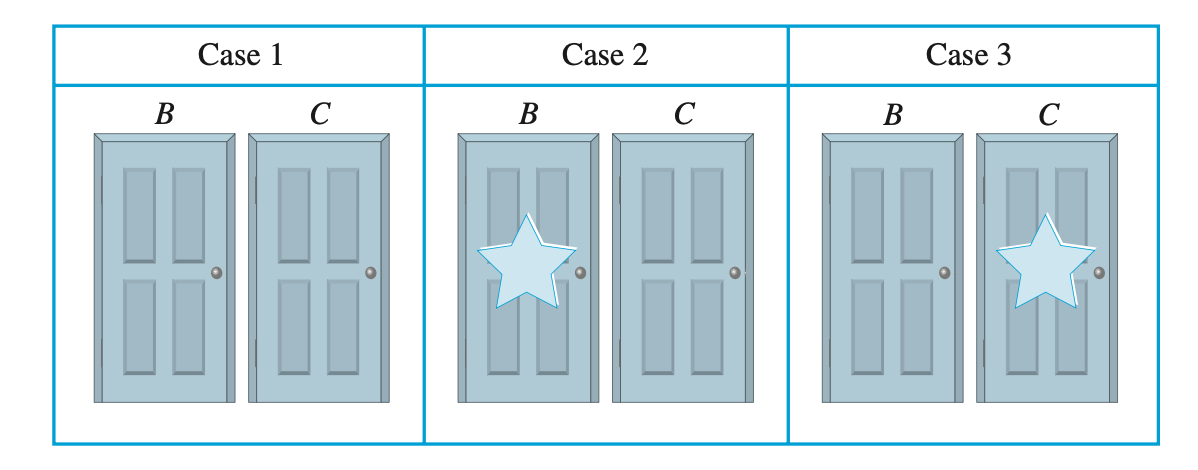
\includegraphics[width=.4\textwidth]{images/monte_hall_solution}
\end{center}

Just before the host opens one of the closed doors, there is no information about the location of the prize. Call the door you pick A.  There are three equally likely possibilities for what lies behind the doors: 
\vspace{-0.2cm}
\begin{itemize}
\item 	(Case 1) The prize is behind A. Here the host could open either door. You would \textbf{win by staying} with your original choice: door A.
\item (Case 2)  The prize is behind B.  Here, the host must open door C, and so you would \textbf{win by switching} to door B.
\item (Case 3)  The prize is behind C.  Here, the host must open door B, and so you would \textbf{win by switching} to door C.
\end{itemize}
%
 Thus, in two of the three equally likely cases, you would win by switching. %from A to the other closed door. %Therefore, you should switch. 
% How to test
\end{frame}

\begin{frame}{The probability of multiple events: Conner's observation}
\small 
\colorbox{blue!30}{\textbf{Review.}} Last time, we  found the probability of drawing the hand $H=\set{6 \clubsuit, K \heartsuit, 3 \diamondsuit, A \spadesuit, 7 \clubsuit}$ in poker as $P(H) = \frac{1}{\binom{52}{5}} = \frac{1}{2,598,960}.$
\vfill 
\pause 
\colorbox{blue!30}{\textbf{Remark.}} We can connect this to Conner's solution via factorial math:
\[P(H)  = \frac{1}{\binom{52}{5}}   = \frac{1}{\frac{52!}{5!47!}} = \frac{5!}{(52)_5} = \frac{5}{52} \cdot \frac{4}{51}  \cdot \frac{3}{50} \cdot \frac{2}{49} \cdot \frac{1}{48} \]
\vfill 
\pause 
\colorbox{yellow!30}{\textbf{Poll.}} How to think of this probabilistically?
\vfill 
\pause 
\colorbox{blue!30}{\textbf{Remark.}} Unraveling the def. of cond'l prob, we obtain the \alert{chain rule}
\[P(A \cap B) = P(A \mid B) P(B) \] 
More generally
\[P(A_1 \cap A_2 \cap \cdots \cap A_n) = P(A_1) P(A_2 \cond A_1) \cdots P(A_n \cond A_1,\cdots A_{n-1}).\]

\vfill 
\pause 
\colorbox{green!30}{\textbf{Solution.}} Here let $A_i$ be the event that the $i$-th card belongs to  $\set{6 \clubsuit, K \heartsuit, 3 \diamondsuit, A \spadesuit, 7 \clubsuit}.$
\end{frame}



\begin{frame}[standout]
Mini-lecture: Independence
\end{frame}

\begin{frame}

\begin{myredbox}[title=\text{Practice Reading Quiz (Conditional Probability and Independence)}]
Let $A$ and $B$ be events in a probability space $(S,P)$.  Under what condition does the below equation hold?
\begin{align}
P(A \cap B) = P(A) \, P(B)
\label{eqn:independence}
\end{align}
\end{myredbox}
\vfill 

\pause 
\begin{mygreenbox}[title=\text{Three characterizations of independence}]

Let $A$ and $B$ be events in a sample space. Here are three equivalent ways to check whether these events are \textbf{independent}:

\begin{enumerate}
	\item $P(A \mid B) = P(A)$
	\item $P(B \mid A) = P(B)$
	\item $P(A \cap B) = P(A) \, P(B)$
\end{enumerate} 
\end{mygreenbox}

\vfill 
\pause 
\begin{myyellowbox}[title=\text{Poll: What do you think about this answer?}]

\Eqref{eqn:independence} holds  when $P(A)$ and $P(B)$ have the same probability of happening.  E. g. $P(A)=1/2$ and $P(B)=1/2$.
\end{myyellowbox}

\end{frame}

\begin{frame}
\small 
\colorbox{yellow!30}{\textbf{Subpoll.}}   Consider the two scenarios below, where we represent probabilities as areas.  In both cases $P(A)=P(B) = \frac{1}{16}$. But in one case $A,B$ are independent, and in the other they are dependent.  Which is which?  Why?

\vfill 

\begin{minipage}{.45\textwidth}


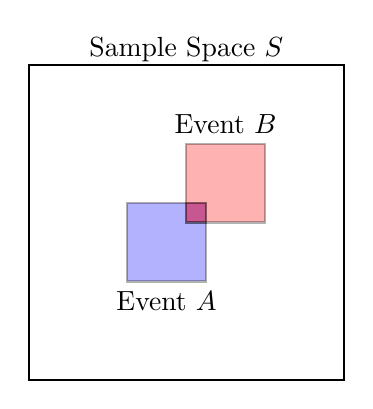
\begin{tikzpicture}

% Draw the sample space S as a large square
\draw[thick] (0,0) rectangle (4,4);
\node at (2, 4.2) {Sample Space \( S \)};

% Draw event A as a smaller square inside S
\draw[thick, fill=blue, opacity=0.3] (1.25, 1.25) rectangle (2.25, 2.25);
\node at (1.75, 1.0) {Event \( A \)};

% Draw event B as another smaller square inside S
\draw[thick, fill=red, opacity=0.3] (2, 2) rectangle (3, 3);
\node at (2.5, 3.25) {Event \( B \)};

% Show intersection area A ∩ B
\draw[thick, fill=purple, opacity=0.3] (2, 2) rectangle (2.25, 2.25);
%\node at (2, 2) {\small $A \cap B$};

\end{tikzpicture}
\end{minipage} %
\hfill 
\begin{minipage}{.45\textwidth}

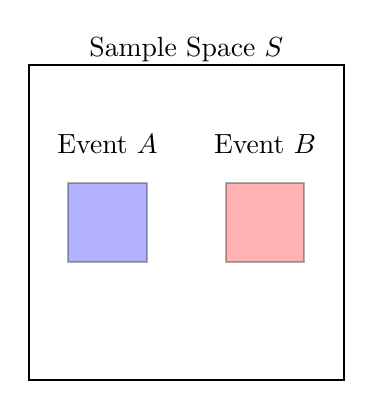
\begin{tikzpicture}

% Draw the sample space S as a large square
\draw[thick] (0,0) rectangle (4,4);
\node at (2, 4.2) {Sample Space \( S \)};

% Draw event A as a smaller square inside S
\draw[thick, fill=blue, opacity=0.3] (0.5, 1.5) rectangle (1.5, 2.5);
\node at (1, 3) {Event \( A \)};

% Draw event B 
\draw[thick, fill=red, opacity=0.3] (2.5, 1.5) rectangle (3.5, 2.5);
\node at (3, 3) {Event \( B \)};

%% Show intersection area A ∩ B
%\draw[thick, fill=purple, opacity=0.3] (1.5, 1.5) rectangle (2.5, 2.5);
%\node at (2, 2) {$A \cap B$};

\end{tikzpicture}
\end{minipage} %

\vfill 
\pause 

\begin{minipage}{.45\textwidth}
\begin{center}
These events are \textbf{independent}.

\begin{align*}
P(A \cap B) &= P(A) \; P(B) \\
&= \frac{1}{16} \cdot \frac{1}{16}   = \frac{1}{256} 
\end{align*}
\end{center}
\end{minipage} %
\hfill 
\pause 
\begin{minipage}{.45\textwidth}

These events are \textbf{dependent}.

\begin{align*}
P(A \cap B) &= 0  \\
& \neq  P(A) \; P(B) = \frac{1}{16} \cdot \frac{1}{16}
\end{align*}
\end{minipage} %
\vfill 
\pause 
\colorbox{orange!30}{\textbf{Remark.}} Dependence doesn't need to be so extreme. The left  figure would depict dependence even if we just pulled the blue and red squares apart from each other ever so slightly.  Likewise if we pushed them closer together slightly.
\end{frame}



\begin{frame}[standout]
Group exercises
\end{frame}


\begin{frame}{Group exercises}

\begin{enumerate}
	\item Let $(S,P)$ be the sample space with $S=\set{1,2,\hdots, 10}$ and $P(x) =\frac{1}{10}$ for all $x \in S$.  Let $A$ be the event \enquote{is even} and $B$ be the event \enquote{is prime}.  Please calculate the following:
	\vspace{-0.5cm}
    \begin{columnsonlytextwidth}
    \begin{column}[t]{0.22\textwidth}
        \begin{itemize} \small
		\item[a.)] $P(A)$ 
		\item[b.)] $P(B)$
        \end{itemize}
    \end{column}
    \begin{column}[t]{0.22\textwidth}
        \begin{itemize} \small
      	\item[c.)] $P(A \cond B)$
		\item[d.)] $P(B \cond A)$ 
        \end{itemize}
    \end{column}
     \begin{column}[t]{0.22\textwidth}
        \begin{itemize} \small
		\item[e.)] $P(\overline{B} \cond A)$ 
		\item[f.)] $P(B \cond \overline{A})$
        \end{itemize}
    \end{column}
    \begin{column}[t]{0.22\textwidth}
        \begin{itemize} \small
		\item[g.)] $P(\overline{B} \cond \overline{A})$. 
        \end{itemize}
    \end{column}
    \end{columnsonlytextwidth}
    \vspace{.2cm}
     Are the events $A$ and $B$ independent?
\item A card is drawn from a well-shuffled deck of 52-cards.
	\begin{itemize}
	\item[a.] What is the probability that it is a spade ($\spadesuit$)?
	\item[b.] What is the probability that it is a king?	
	\item[c.] What is the probability that it is the king of spades?
	\item[d.] Are the events in parts (a) and (b) independent?
	\end{itemize}
\item Solve the spinner winner problem (see next slide).
\item Prove Scheinerman Prop. 32.4.
\item Let $A$ and $B$ be events in a sample space with $P(A \cap B) \neq 0$.  Prove that $P(A \cond B) = P(B \cond A)$ if and only if $P(A) = P(B)$.
\end{enumerate}

\end{frame}


\begin{frame}

\begin{figure}
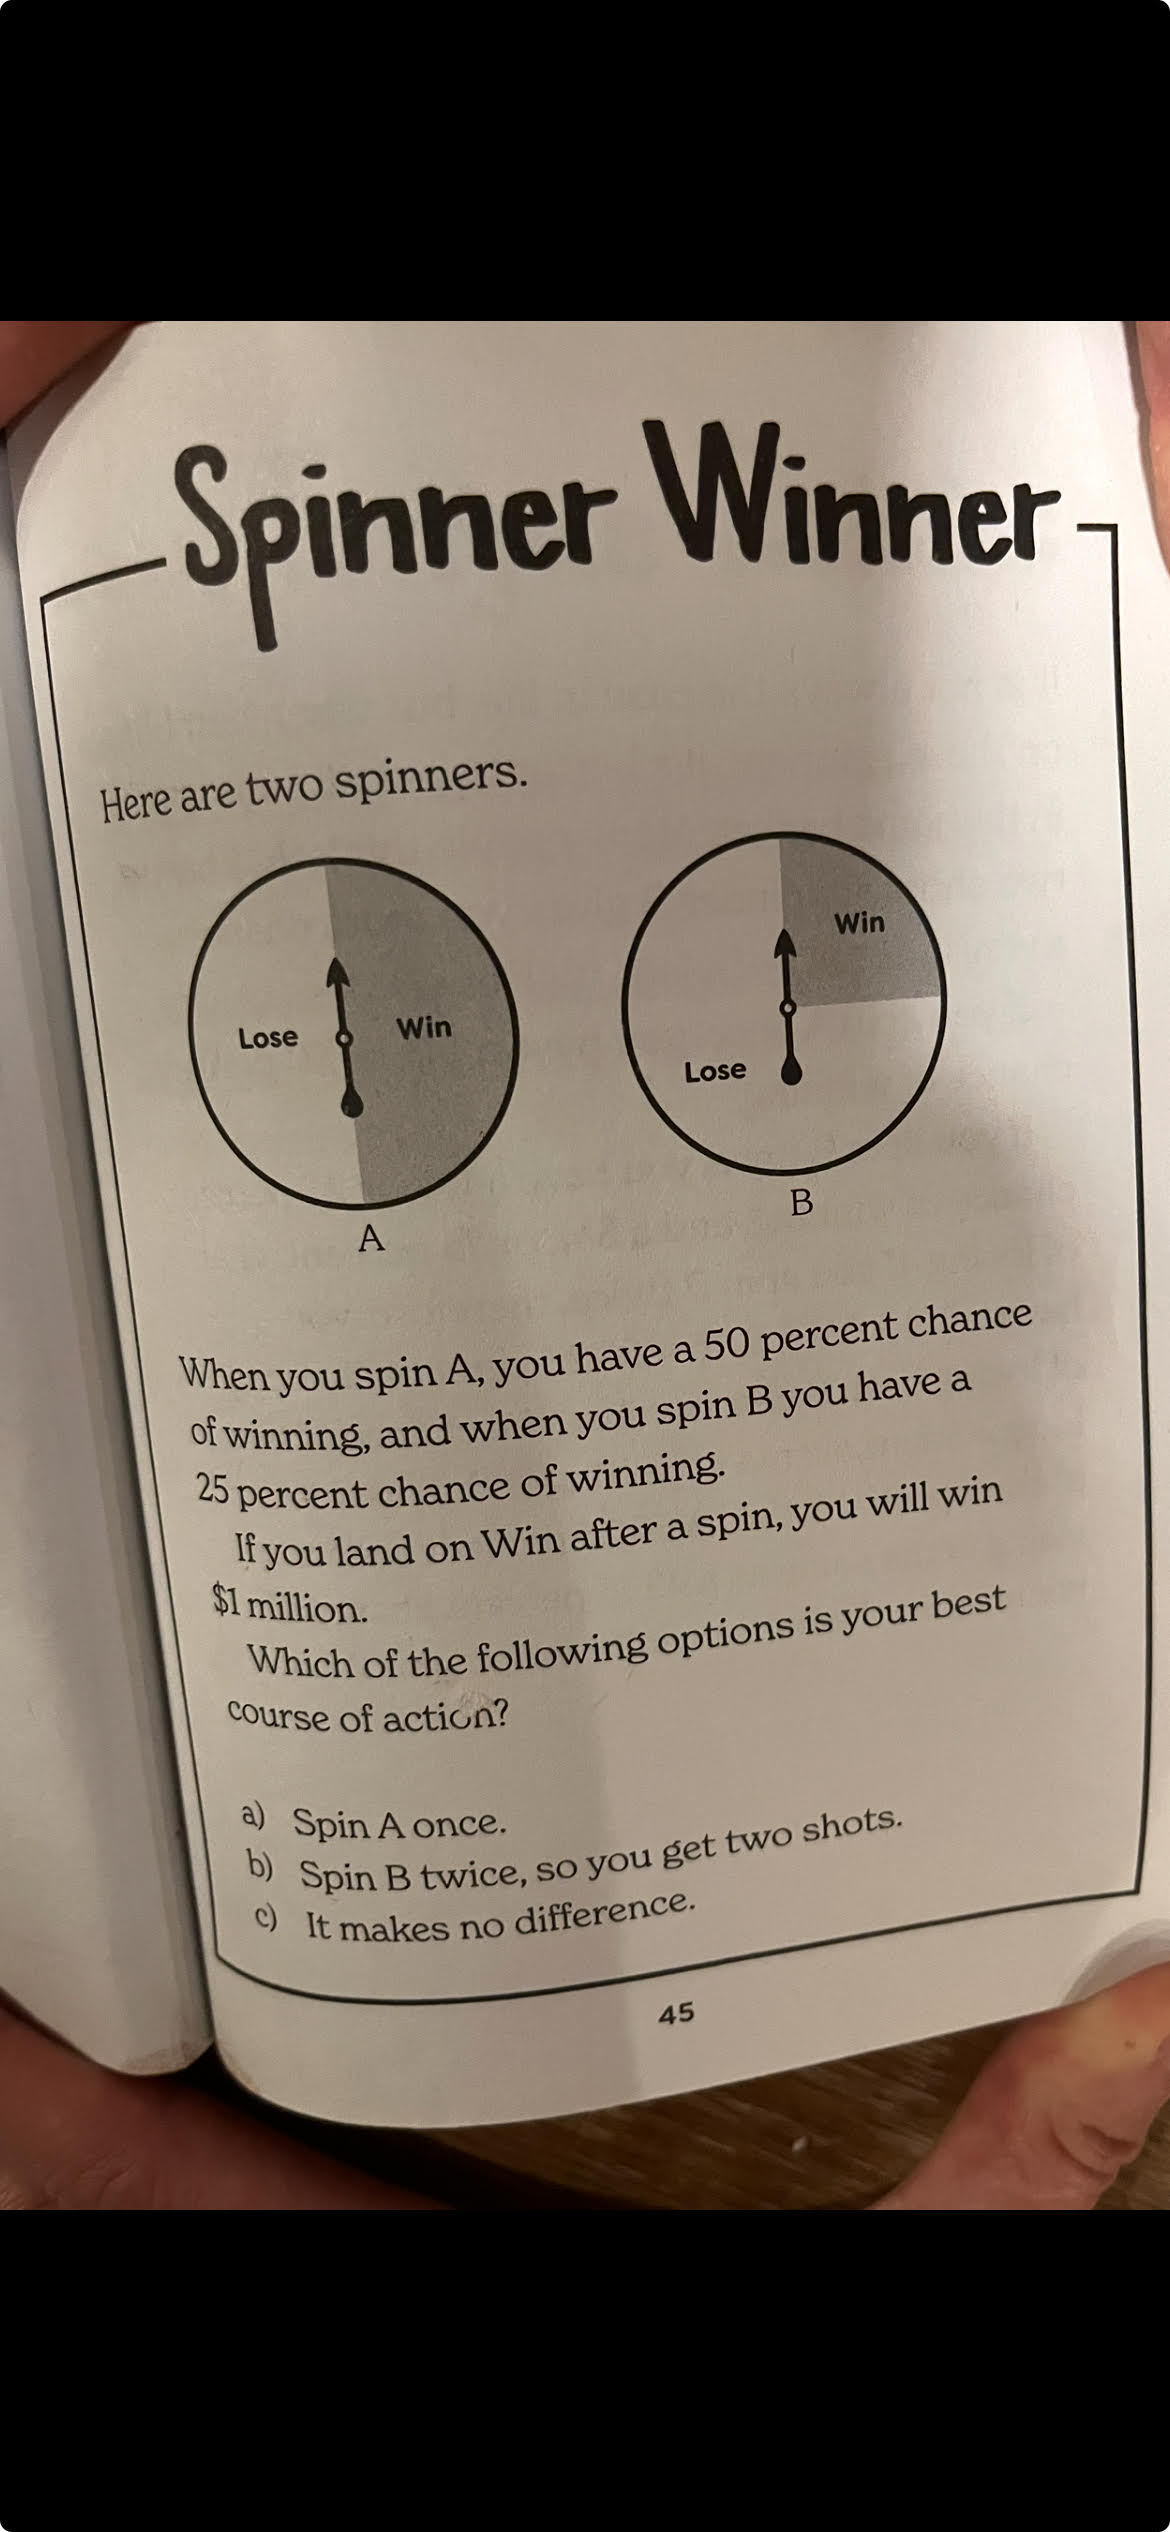
\includegraphics[width=.5\textwidth]{images/spinner_winner.jpg}	
\end{figure}

\end{frame}



\begin{frame}{Solution to group exercise \#1a,b,c,d}
\footnotesize 
\vspace{-.1cm} 
\textbf{Problem.}  Let $(S,P)$ be the sample space with $S=\set{1,2,\hdots, 10}$ and $P(x) =\frac{1}{10}$ for all $x \in S$.  Let $A$ be the event \enquote{is even} and $B$ be the event \enquote{is prime}.  Please calculate the following: (a) $P(A)$,  (b) $P(B)$, (c) $P(A \cond B)$, (d) $P(B \cond A)$. Also determine if $A$ and $B$ are independent.

\vspace{-.135cm}
\textbf{Solution.}
We have 
\[
\begin{array}{r@{}l r@{}l}
S &= \set{1,2,\hdots, 10} & |S| &= 10 \\
A &= \set{2,4,6,8,10} & |A| &= 5 \\
B &= \set{2,3,5,7} & |B| &= 4 \\
A \cap B &= \set{2} & |A \cap B| &= 1
\end{array}
\]
%
By the equally likely probability formula, we have
 \[ P(A) = \frac{|A|}{|S|} = 5/10, \qquad P(B) = \frac{|B|}{|S|} = 4/10, \qquad P(A \cap B) =  \frac{|A \cap B|}{|S|} = 1/10. \]
Hence,
\[P(A \cond B) = \frac{P(A \cap B)}{P(B)} = \frac{1/10}{4/10} = 1/4, \qquad  P(B \cond A) = \frac{P(A \cap B)}{P(A)} = \frac{1/10}{5/10} = 1/5.\]
These events are not independent, since $P(A \cap B) \neq P(A) P(B).$

%
\vspace{-.135cm} 
\textbf{Interpretation}: $P(A \cond B)$ gives the probability of randomly drawing an even number from the prime numbers in $S$.  It makes sense that $P(A \cond B)=1/4$: looking at set $B$, there are 4 prime numbers in $S$, only one of them is also even, and all of these numbers are equally likely to be drawn.  Similarly, $P(B \cond A)$ gives the probability of randomly drawing a prime number from the even numbers in $S$.  Note there are 5 even numbers, and only one of them is prime. 
\end{frame}


\begin{frame}{Solution to group exercise \#1e,f,g}
\footnotesize 
\textbf{Problem.}  Let $(S,P)$ be the sample space with $S=\set{1,2,\hdots, 10}$ and $P(x) =\frac{1}{10}$ for all $x \in S$.  Let $A$ be the event \enquote{is even} and $B$ be the event \enquote{is prime}.  Please calculate the following: (e) $P(\overline{B} \cond A)$, (f) $P(B \cond \overline{A})$, (g) $P(\overline{B} \cond \overline{A})$.
		
\vfill 

\textbf{Solution.}
We have 
\[
\begin{array}{r@{}l r@{}l}
S &= \set{1,2,\hdots, 10} & |S| &= 10 \\
\overline{A} &= \set{1,3,5,7,9} & |\overline{A}| &= 5 \\
\overline{B} &= \set{1,4,6,8,9,10} & |\overline{B}| &= 6 \\
A \cap \overline{B} &= \set{4,6,8,10} & |A \cap \overline{B}| &= 4 \\
\overline{A} \cap B &= \set{3,5,7} & |\overline{A} \cap B | &= 3 \\
\overline{A} \cap \overline{B} &= \set{1,9} & |\overline{A} \cap  \overline{B} | &= 2
\end{array}
\]
%
We have 
%
\begin{align*}
P(\overline{B} \cond A) &= \frac{\overline{B} \cap A}{P(A)} = \frac{4/10}{5/10} = 4/5. \\
P(B \cond \overline{A}) &= \frac{B \cap \overline{A}}{P(\overline{A})} = \frac{3/10}{5/10} = 3/5 \\
P(\overline{B} \cond \overline{A}) &= \frac{\overline{B} \cap \overline{A}}{P(\overline{A})} = \frac{2/10}{5/10} = 2/5.
\end{align*}
%
\vfill 
\textbf{Example Interpretation}: $P(B \cond \overline{A})$ gives the probability of randomly drawing a prime number from the odd (non-even) numbers in $S$.  Looking at $\overline{A}$, we see that there are 5 odd numbers (all of them equally likely to be drawn), and 3 of them are prime.
\end{frame}


\begin{frame}{Solution to group exercise \#2}


\textbf{Problem.} A card is drawn from a well-shuffled deck of 52-cards.
	\begin{itemize}
	\item[a.] What is the probability that it is a spade ($\spadesuit$)?
	\item[b.] What is the probability that it is a king?	
	\item[c.] What is the probability that it is the king of spades?
	\item[d.] Are the events in parts (a) and (b) independent?
	\end{itemize}
\vfill 
\textbf{Solution.} Let $A$ be the event \enquote{is a spade} and $B$ be the event \enquote{is king}. By the equally likely probability formula,
	\begin{itemize}
	\item[a.] $P(A) = \frac{|A|}{|S|} = \frac{13}{52} = \frac{1}{4}.$
	\item[b.] $P(B) = \frac{|B|}{|S|} = \frac{4}{52} = \frac{1}{13}.$	
	\item[c.] $P(A \cap B) = \frac{|A \cap B|}{|S|} = \frac{1}{52} = \frac{1}{52}.$	
	\item[d.] Yes. Note that 
	\[ \frac{1}{52} = P(A \cap B) =P(A) \times P(B) = \frac{1}{4} \times \frac{1}{13} \]
	so the definition of independent events is verified.  Intuitively, the suit of a card (e.g. spade) provides no information about its rank (e.g. king). 
	\end{itemize}

\end{frame}

\begin{frame}{Solution to group exercise \#3}

If you spin $A$, you have a 50\% chance of winning.

If you spin $B$ twice, then you win the money if you win on the first spin $W_1$ \textbf{or} if you win on the second spin $W_2$.

Now, by the general addition rule

\[
P(W_1 \cup W_2) = P(W_1) + P(W_2) - P(W_1 \cap W_2)	
\]
%
Moreover, since the spins are independent, we have $P(W_1 \cap W_2) = P(W_1) P(W_2)$.   So all together

\begin{align*}
P(W_1 \cup W_2) &= P(W_1) + P(W_2) - P(W_1) P(W_2) \\
&= \frac{1}{4} + \frac{1}{4} - \bigg(\frac{1}{4} \cdot \frac{1}{4}\bigg) \\
&= \frac{1}{2} - \frac{1}{16}\\
&=.4357	
\end{align*}

So it's better to spin $A$.

\end{frame}



\begin{frame}{Solution to group exercise \#4}
\small 
\textbf{Problem.} Prove Scheinerman Prop. 32.4.
\vfill 
\textbf{Solution.} 
\begin{itemize}
\item $\boxed{(3) \implies (1).}$
\[ P(A \cond B) \stackexplain{def.}{=}	 \frac{P(A \cap B)}{P(B)} \stackexplain{(3)}{=}	   \frac{P(A) \cancel{P(B)}}{\cancel{P(B)}} = P(A).  \]
\item $\boxed{(3) \implies (2).}$
\[ P(A \cond B) \stackexplain{def.}{=}	 \frac{P(A \cap B)}{P(A)} \stackexplain{(3)}{=}	   \frac{ \cancel{P(A)} P(B)}{\cancel{P(A)}} = P(B).  \]
\item $\boxed{(1) \implies (3).}$
\[ P(A \cap B) \stackexplain{def.}{=}	  P(A \cond B) P(B) \stackexplain{(1)}{=}	P(A) P(B) \]
\item $\boxed{(2) \implies (3).}$
\[ P(A \cap B) \stackexplain{def.}{=}	  P(B \cond A) P(A) \stackexplain{(2)}{=}	P(B) P(A) \]
\end{itemize}
In the above, \enquote{\textit{def.}} refers to the definition of conditional probability.
\end{frame}


\begin{frame}{Solution to group exercise \#5}
\small 
\textbf{Problem.} Let $A$ and $B$ be events in a sample space with $P(A \cap B) \neq 0$.  Prove that $P(A \cond B) = P(B \cond A)$ if and only if $P(A) = P(B)$.
\vfill 
\vspace{-.1cm}
\textbf{Remark.} Recall that to prove an \enquote{if and only if} statement, we must prove that if-then propositions hold in both directions. 
\vfill 
\vspace{-.1cm}
\textbf{Solution.}
\begin{itemize}
\item $\boxed{\implies}$. We assume $P(A \cond B) = P(B \cond A)$  and show $P(A) = P(B)$.   Since $P(A \cond B) = P(B \cond A)$, by the definition of conditional probability, we have
\[ \frac{P(A \cap B)}{P(A)} =  \frac{P(A \cap B)}{P(B)}.\] 
 Cross multiplying, we obtain
 \[ P(A \cap B) \, P(A) =  P(A \cap B) \, P(B). \]
 Since $P(A \cap B) \neq 0$, we can divide both sides by it, leaving $P(A)=P(B)$. %(and $P(A \cap B) \neq 0$)
\item $\boxed{\impliedby}$. We assume $P(A) = P(B)$ and show $P(A \cond B) = P(B \cond A)$.   We have
%
\begin{align*}
P(A \cond B) 	\stackexplain{def.}{=}	 \frac{P(A \cap B)}{P(B)} \stackexplain{assumpt.}{=}	\frac{P(A \cap B)}{P(A)}\stackexplain{def.}{=}	P(B \cond A). 
\end{align*}

\end{itemize}

\end{frame}


\end{document}
